%==============================================================================
% Report, Part A only: PCM write-absorbing tier for an HBM + HBF KV cache.
%
% Source: Documents/Report/report.md, Part A (sections A1-A9), as of
% 2026-10-22. Part B (working record) is not included. If this file and
% TokenSim/docs/findings.md disagree, findings.md wins.
%
% Bibliography entries are copied from pcm-kv-micro.tex (verified 2026-10-22).
%
% Build:  pdflatex report-partA.tex  (run twice for the contents and refs)
% Packages: all from a standard TeX Live install (xltabular, booktabs,
% enumitem, tikz, url, hyperref, caption, etoolbox, microtype, lmodern).
%==============================================================================
\documentclass[11pt,a4paper]{article}

\usepackage[T1]{fontenc}
\usepackage[utf8]{inputenc}
\usepackage{lmodern}
\usepackage{microtype}
\usepackage[margin=25mm]{geometry}
\usepackage{amsmath}
\usepackage{array}
\usepackage{booktabs}
\usepackage{xltabular}
\usepackage{etoolbox}
\usepackage{enumitem}
\usepackage{xcolor}
\usepackage{tikz}
\usetikzlibrary{arrows.meta,positioning}
\usepackage[font=small,labelfont=bf]{caption}
\usepackage{url}
\usepackage[hidelinks]{hyperref}

% Section numbering A1, A2, ...; subsections are unnumbered, as in report.md.
\renewcommand{\thesection}{A\arabic{section}}
\setcounter{secnumdepth}{1}
\setcounter{tocdepth}{1}

% Code identifiers and file paths: typewriter, breakable at _ . : - / , =
\urlstyle{tt}
\makeatletter
\def\UrlBreaks{\do\_\do\.\do\:\do\-\do\/\do\,\do\=}
\makeatother
\Urlmuskip=0mu plus 1mu

% Tables: small type, a little extra row height, ragged-right X columns.
\AtBeginEnvironment{xltabular}{\small\renewcommand{\arraystretch}{1.15}}
\newcolumntype{L}{>{\raggedright\arraybackslash}X}
\newcolumntype{Y}[1]{>{\raggedright\arraybackslash\hsize=#1\hsize}X}
\newcolumntype{P}[1]{>{\raggedright\arraybackslash}p{#1}}
\newcommand{\hd}[1]{\textbf{#1}}

\setlist{itemsep=2pt,topsep=4pt,parsep=0pt}
\setlength{\parskip}{4pt}
\setlength{\parindent}{0pt}

\newcommand{\CT}{Conv\,/\,T\&A}
\newcommand{\OPEN}{\textbf{OPEN}}

\begin{document}

%==============================================================================
\begin{center}
  {\LARGE\bfseries PCM Write-Absorbing Tier for an\\[2pt]
   HBM\,+\,HBF KV Cache}\\[8pt]
  {\large Report --- Part A}\\[10pt]
  Rishabh Chamoli\\
  Indian Institute of Technology Guwahati\\[4pt]
  Last updated: 22 October 2026
\end{center}

\begin{xltabular}{\linewidth}{@{}P{30mm} L@{}}
\toprule
Simulator & \path{TokenSim/} (SimPy LLM-serving simulator with a Mooncake KV store) \\
Full record & \path{TokenSim/docs/findings.md} (append-only). If this report and findings.md disagree, findings.md wins \\
Latest phase & \textbf{PHASE 14} (full-trace headline, HBF capacity check, break-even PCM endurance) \\
Tests & \textbf{277} passing \\
\bottomrule
\end{xltabular}

\textbf{Conventions.} Anything marked \OPEN{} is an unsourced parameter.
Anything marked \textbf{ASSUMED} or \textbf{PLACEHOLDER} is used or recorded
but not sourced.

\tableofcontents

%==============================================================================
\section{The question}\label{sec:question}
%==============================================================================

\textbf{H3}~\cite{h3} (SK hynix, IEEE CAL 2026) adds high-bandwidth flash
(HBF, NAND) behind HBM.

\begin{itemize}
  \item H3 targets \textbf{read-only} data: model weights and shared,
    precomputed KV. For that data, NAND's low write endurance does not matter.
  \item \textbf{We put the same hardware under a write-heavy serving
    workload.} Here KV blocks evicted from HBM are spilled to HBF, so HBF
    receives a continuous write stream and its endurance is at risk.
\end{itemize}

We add a \textbf{bit-alterable non-volatile tier (PCM)} between HBM and HBF
and ask \textbf{how much of the HBF write stream it can absorb, and at what
cost in reuse.}

%==============================================================================
\section{The architecture being modelled}\label{sec:arch}
%==============================================================================

\subsection{Per-GPU hardware}

\begin{xltabular}{\linewidth}{@{}P{24mm} Y{1.15} Y{0.85}@{}}
\caption{Per-GPU hardware.}\label{tab:hw}\\
\toprule
\hd{tier} & \hd{capacity per GPU} & \hd{source} \\
\midrule
HBM3e & 192\,GB, 8 cubes $\times$ 24\,GB, all KV (weights live in HBF) & H3~\cite{h3} \\
HBF (NAND, TLC) & 3\,TB, 8 stacks $\times$ 384\,GB, 3000 P/E & H3 (capacity); CLAUDE.md (P/E) \\
PCM (our addition) & \textbf{43.4\,GiB}: 2 dies/stack $\times$ 35\,mm$^2$ $\times$ 0.62\,Gb/mm$^2$ = 43.4\,Gb = 5.43\,GiB per stack, $\times$ 8 stacks
  & 0.62\,Gb/mm$^2$: 1st-gen 3D XPoint, Ehrmann \emph{et al.}, \emph{Applied Research} 2022~\cite{ehrmann2022pcm} \\
\bottomrule
\end{xltabular}

\begin{itemize}
  \item \textbf{Topology.} HBM and HBF are daisy-chained through a router in
    the HBM base die; no HBM is given up for flash (H3).
  \item \textbf{PCM placement.} PCM sits \textbf{on top of each HBF stack,
    inside the existing footprint}, so it takes no NAND capacity.
  \item \textbf{Units.} Binary throughout: Gb = $2^{30}$ bits, GB read as GiB.
\end{itemize}

\subsection{Data path}

\begin{center}
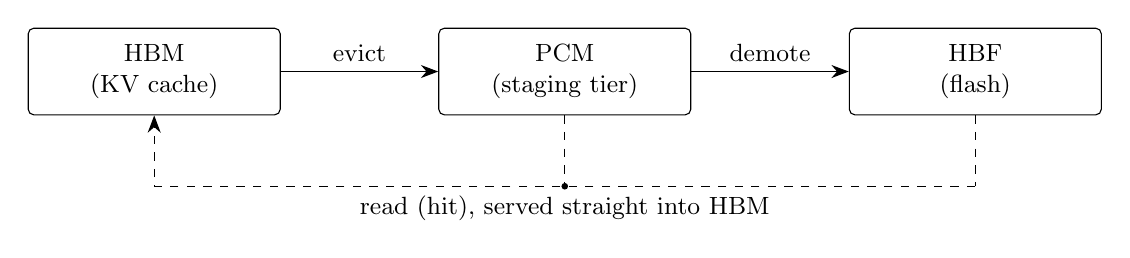
\begin{tikzpicture}[
    box/.style={draw, rounded corners=2pt, minimum width=32mm,
                minimum height=11mm, align=center, font=\small},
    >={Stealth[length=2.2mm]}, node distance=20mm]
  \node[box] (hbm) {HBM\\(KV cache)};
  \node[box, right=of hbm] (pcm) {PCM\\(staging tier)};
  \node[box, right=of pcm] (hbf) {HBF\\(flash)};
  \draw[->] (hbm) -- node[above, font=\small] {evict} (pcm);
  \draw[->] (pcm) -- node[above, font=\small] {demote} (hbf);
  \draw[dashed] (hbf.south) -- ++(0,-9mm) coordinate (r);
  \draw[dashed, ->] (r) -| node[pos=0.25, below, font=\small]
      {read (hit), served straight into HBM} (hbm.south);
  \draw[dashed] (pcm.south) -- (pcm.south |- r);
  \fill (pcm.south |- r) circle (1.2pt);
\end{tikzpicture}
\end{center}

\begin{itemize}
  \item \textbf{A block enters the store only when HBM evicts it} (spill).
  \item \textbf{On a later request, a block is read from PCM or HBF straight
    into HBM.} An HBF hit is \textbf{not} re-admitted to PCM: \path{store.get}
    reads it in place (\path{store.py:179-182}), and a later spill of the same
    key only refreshes it (\path{store.py:234-237}).
  \item \textbf{When PCM is full}, its LRU victim is either demoted to HBF or
    dropped, depending on the configuration.
\end{itemize}

\subsection{The three configurations}

\begin{xltabular}{\linewidth}{@{}l Y{0.8} Y{1.0} Y{1.0} Y{1.2}@{}}
\caption{The three configurations.}\label{tab:configs}\\
\toprule
 & \hd{staging tier} & \hd{admission write} & \hd{at staging-tier eviction} & \hd{what it represents} \\
\midrule
\textbf{(b)} & 71,104-block \textbf{DRAM} buffer
  & \textbf{write-through}: the block also goes to HBF immediately
  & demote to HBF (\path{always})
  & \textbf{the baseline}. Not ``HBF only'': the buffer serves 6.9\%\,/\,7.2\% of (b)'s store-served tokens \\
\textbf{(c)} & 71,104-block \textbf{PCM}
  & \textbf{write-back}: PCM only
  & demote to HBF (\path{always})
  & removes the write-through copy \\
\textbf{(d)} & 71,104-block \textbf{PCM}
  & \textbf{write-back}
  & demote \textbf{only if the block was served from PCM at least once} (\path{if_read}), otherwise drop
  & \textbf{read-gated demotion}: our policy \\
\bottomrule
\end{xltabular}

Every number below is quoted as \textbf{\CT}, i.e.\ Mooncake Conversation
trace\,/\,Tool\&Agent trace.

%==============================================================================
\section{How it is simulated}\label{sec:sim}
%==============================================================================

\subsection{Simulator}

\textbf{TokenSim}~\cite{tokensim} is an event-driven (SimPy) LLM-serving
simulator. Its \textbf{Mooncake store}~\cite{mooncake} has a memory tier and
an offload tier, each with LRU eviction.

\begin{xltabular}{\linewidth}{@{}P{45mm} L@{}}
\caption{Tier roles in TokenSim.}\label{tab:roles}\\
\toprule
\hd{tier} & \hd{role} \\
\midrule
HBM & the GPU prefix cache \\
Mooncake memory tier & the staging tier (PCM, or DRAM in (b)) \\
Mooncake offload tier & HBF \\
\bottomrule
\end{xltabular}

\begin{itemize}
  \item Each tier is a \textbf{per-operation latency function},
    $\text{latency} = \text{fixed}_{\mu s} + \text{bytes} / \text{bandwidth}$
    (\path{mooncake/ssd.py}).
  \item Bandwidth is not shared between operations, and there is no queueing
    model for the far tier.
  \item \textbf{Write volume is counted exactly, in blocks and bytes, per
    tier.}
\end{itemize}

All PHASE 14 behaviour is added behind configuration flags whose default is
the stock behaviour. With every flag at its default, output is byte-identical
to the pre-PHASE-14 code (\path{ced3806}).

\subsection{Model and block size}

\begin{xltabular}{\linewidth}{@{}P{30mm} Y{1.15} Y{0.85}@{}}
\caption{Model and block size.}\label{tab:model}\\
\toprule
\hd{quantity} & \hd{value} & \hd{source} \\
\midrule
model & LLaMa2-70B-GQA: $N_\text{head}$ 64, KV heads 64/8 = \textbf{8}, $N_\text{layer}$ 80, $D_\text{model}$ 8192, head dim 128
  & \path{hardware_models_h3b200.json:566-572} \\
precision & \textbf{FP16, hardcoded} (2 bytes per value) & \path{cache_config.py:46-52} \\
parallelism & TP2\,/\,PP1\,/\,DP4 on 8 GPUs. TP2 splits KV heads: \textbf{4 per shard} & \path{cache_config.py:173-178} \\
KV bytes per token, per TP shard & 4 heads $\times$ 128 $\times$ 2 (K,V) $\times$ 2\,B $\times$ 80 layers = \textbf{163,840\,B} & \path{cache_config.py:46-52} \\
tokens per block & 16 & \path{--block_size}\texttt{ }\path{16} \\
\textbf{bytes per block} & 16 $\times$ 163,840 = \textbf{2,621,440\,B}
  & \path{mooncake_store.py:41-43}. Measured: bytes $\div$ blocks = 2,621,440 in every run \\
\bottomrule
\end{xltabular}

\textbf{Cross-check.} 43.4\,GiB per GPU $\div$ 2,621,440\,B = 17,776.64
blocks, floored to \textbf{17,776}. So the configured PCM is 17,776 $\times$
2,621,440\,B = 43.398\,GiB per GPU, agreeing with the design to within the
floor (+0.0036\%).

\textbf{FP16 is a limitation.} FP8 would halve every byte count and double
every tier's capacity in blocks.

\subsection{Capacity bookkeeping: writing ranks and private pools}

\begin{itemize}
  \item \textbf{Only 4 of the 8 GPUs write to the store.} Only the TP-0
    worker of each data-parallel group is scheduled
    (\path{llm_engine.py:577-579}). The TP-1 shard's stream is an exact
    mirror and is not simulated.
  \item \textbf{Every byte figure is therefore per TP shard} (one of 2).
    Ratios and reductions are unaffected.
  \item \textbf{Batch is quoted per active scheduler} =
    \path{batch_mean_cluster} $\div$ 4.
  \item \textbf{Pools are sized for the 4 writing GPUs and split into 4
    private partitions} (\path{store_partition}\texttt{ }\path{=}\texttt{ }\path{per_rank}). PCM is
    in-package on each GPU's own HBF stacks, so one GPU cannot evict
    another's blocks.
\end{itemize}

\begin{xltabular}{\linewidth}{@{}l Y{1.0} Y{0.8} Y{1.0} Y{1.2}@{}}
\caption{Pool sizing per tier.}\label{tab:pools}\\
\toprule
\hd{tier} & \hd{pool knob} & \hd{split in code} & \hd{per writing GPU} & \hd{recorded in every result} \\
\midrule
PCM & \path{memory_capacity_blocks}\texttt{ }\path{=}\texttt{ }\path{71,104} & \path{71,104}\texttt{ }\path{//}\texttt{ }\path{4} (\path{store.py:446})
  & \textbf{17,776 blocks = 43.4\,GiB} & \path{partition_rank_memory_capacity_blocks}\texttt{ }\path{=}\texttt{ }\path{17,776} \\
HBF & \path{ssd_capacity_blocks}\texttt{ }\path{=}\texttt{ }\path{5,033,164} & \path{5,033,164}\texttt{ }\path{//}\texttt{ }\path{4} (\path{ssd.py:157-158})
  & \textbf{1,258,291 blocks = 3\,TiB} (3,298,534,359,040\,B) & \path{partition_rank_ssd_capacity_blocks}\texttt{ }\path{=}\texttt{ }\path{1,258,291} \\
HBM & from the hardware entry's \path{Capacity} & per GPU & \textbf{78,643 blocks = 192\,GiB} & --- \\
\bottomrule
\end{xltabular}

\textbf{24\,TiB, 12\,TiB and 3\,TiB are all correct; they measure different
things.}
\begin{itemize}
  \item 24\,TiB is the HBF of all 8 GPUs.
  \item 12\,TiB is the HBF of the 4 writing GPUs, which receives the counted
    bytes.
  \item 3\,TiB is one writing GPU's partition.
\end{itemize}

\textbf{HBM \path{Capacity} is pre-compensated by +60.38\,GiB.} TokenSim
subtracts the model weights from HBM, but H3 keeps the weights in HBF. This is
a workaround, not a model change.

\subsection{The headline configuration, and why it was chosen}

{\footnotesize
\begin{verbatim}
memory_capacity_blocks = 71104     ssd_capacity_blocks   = 5033164
store_partition        = per_rank  store_partition_ranks = 4
hbm_evict_save_policy  = spill_only    # a block enters PCM only when HBM evicts it
store_lookup_start     = after_hbm     # look up only the blocks HBM did not hit
read_credit            = served        # if_read credits a block only when PCM served it
load_span              = missing       # load only the span HBM did not hit
cap 48 concurrent requests per scheduler; 30 QPS; full traces
\end{verbatim}
}

\textbf{Capacity and partition were chosen on hardware grounds}
(Section~\ref{sec:arch}, above).

\textbf{Entry, lookup and bookkeeping were chosen on modelling grounds.} This
is the only combination in which the store behaves as the intended hierarchy
and PCM serves real reads. Each alternative fails in a specific, measured way:

\begin{xltabular}{\linewidth}{@{}Y{0.8} Y{1.2} P{26mm}@{}}
\caption{Rejected alternatives to the headline entry, lookup and bookkeeping.}\label{tab:alts}\\
\toprule
\hd{alternative} & \hd{what goes wrong} & \hd{where} \\
\midrule
copy every prompt block into the store at admission (\path{prefill}, stock)
  & HBM and the store become parallel copies, not a hierarchy. PCM never serves a read (0 PCM-served tokens in 332 runs)
  & PHASE 12; PHASE 14 set A \\
spill-only, but the lookup starts at block 0 (\path{zero}, stock)
  & the head of the prompt stays in HBM, so the walk stops at the first absent key. The store serves 0\,/\,769 of 5,000 lookups
  & PHASE 14 STEP 3b \\
\path{read_credit}\texttt{ }\path{=}\texttt{ }\path{walked} (stock)
  & \path{if_read} credited every key the lookup \emph{walked}, including blocks actually served from HBM. That opened the gate with no PCM read
  & PHASE 14 set A; V1 \\
\path{load_span}\texttt{ }\path{=}\texttt{ }\path{from_start} (stock)
  & the load plan read the prompt head, not the span HBM missed (\path{mooncake_store.py:543})
  & PHASE 14 set B \\
\bottomrule
\end{xltabular}

\path{after_hbm} follows the vLLM~\cite{vllm} KV-connector contract:
\path{get_num_new_matched_tokens(request,}\texttt{ }\path{num_computed_tokens)} asks the
external store only for tokens beyond the local hit. We cite the interface
only.

\subsection{Timing knobs (all runs)}

\begin{xltabular}{\linewidth}{@{}P{30mm} Y{0.8} Y{1.2}@{}}
\caption{Timing knobs.}\label{tab:timing}\\
\toprule
\hd{knob} & \hd{value} & \hd{status} \\
\midrule
HBF read & 0.1\,\textmu s, 7451\,GiB/s (= 8\,TB/s)
  & 8\,TB/s from H3. 0.1\,\textmu s is a \textbf{perfect-prefetch upper bound} for H3's latency-hiding buffer. This flatters (b) \\
\textbf{HBF write} & \textbf{200\,\textmu s, 3.0\,GiB/s}
  & \textbf{TokenSim's stock SSD default, unsourced.} These are the values every run used \\
PCM read\,/\,write & 0.1\,/\,1.0\,\textmu s, 100\,/\,20\,GiB/s
  & \textbf{ASSUMED} (TokenSim defaults for the PCM media model) \\
\path{charge_eviction_writes} & true & demote writes are charged to the put that caused them \\
\bottomrule
\end{xltabular}

\begin{itemize}
  \item \textbf{Byte counts are the results; timing only shapes the
    schedule.} PHASE 14 STEP 2 removed all store time, or scaled the PCM
    write timing 0.25$\times$ and 4$\times$. Neither (b)'s HBF stream nor any
    PCM stream moved by more than 0.54\%.
  \item That test ran under the earlier copy-at-admission model and has
    \textbf{not been repeated under the headline}.
\end{itemize}

\subsection{Workload and replay}

\begin{itemize}
  \item \textbf{Traces.} Mooncake FAST'25~\cite{mooncake} Conversation
    (\textbf{12,031 requests}) and Tool\&Agent (\textbf{23,608}), replayed in
    full at \textbf{30 QPS} (\path{--trace_target_qps}\texttt{ }\path{30}).
  \item \textbf{They stand in for CAG} (cache-augmented generation), the H3
    target workload. CAG's corpus size, sharing factor and transient KV are
    \OPEN.
  \item \textbf{Prompt blocks only.} The store holds prompt KV. Generated KV
    has no key and never enters it. Generated tokens are
    \textbf{2.58\%\,/\,1.94\%} of all tokens, which bounds what this omission
    can change on these traces.
  \item \textbf{Hit rates are floors.} The traces hash prompts in 512-token
    chunks, while the simulator uses 16-token blocks. A continuation therefore
    cannot reuse its predecessor's partial tail (PHASE 13).
  \item \textbf{Trace timestamps are whole seconds}, clustered into bursts.
    Order within a burst is file order.
\end{itemize}

\subsection{Replicates}

\begin{itemize}
  \item \textbf{(b) and (c) are single runs.} Their HBF streams vary by
    $\le$\,0.5\% under perturbation, measured in STEP 2b and the STEP 3
    prelude.
  \item \textbf{(d) is $N = 4$ per trace}: the unjittered run, plus 3 runs
    with \textbf{burst-level arrival jitter}, seeds 1--3.
  \begin{itemize}
    \item Each burst is shifted by a random offset of up to
      $j = 0.05 \times$ the minimum inter-burst gap: \textbf{16.989\,ms
      (Conv) and 33.338\,ms (T\&A)}.
    \item The run fails unless arrival order still equals file order.
    \item Every (d) figure is a range over the 4 runs, never a midpoint.
  \end{itemize}
  \item \textbf{\path{--random_seed} is inert} on these traces: seeds 0/1/2
    are byte-identical (PHASE 14 STEP 2b). That is why jitter is used to make
    replicates.
\end{itemize}

\subsection{Metrics}

\begin{xltabular}{\linewidth}{@{}P{42mm} L@{}}
\caption{Metrics.}\label{tab:metrics}\\
\toprule
\hd{metric} & \hd{definition} \\
\midrule
\endfirsthead
\toprule
\hd{metric} & \hd{definition} \\
\midrule
\endhead
\bottomrule
\endlastfoot
\textbf{HBF B/req} & bytes written to HBF $\div$ requests, \textbf{per TP shard}. The primary write metric; it is work-normalised \\
reduction (x)$\to$(y) & $1 - \text{B/req}(y) \div \text{B/req}(x)$ \\
residue-adjusted reduction & adds to HBF bytes the \textbf{end-of-run residue}: keyed blocks still in HBM at the end that were never spilled, assumed eventually demoted. Bounds the end-of-window bias \\
hit rate & prefix-cache hit rate (HBM + store) \\
\textbf{no-store control / store benefit kept} & the same run with the store disabled.
  Benefit kept = $(\mathit{hit} - \mathit{hit}_\text{no-store}) \div (\mathit{hit}_\text{(b)} - \mathit{hit}_\text{no-store})$ \\
PCM-served share & store-served tokens served from PCM $\div$ all store-served tokens \\
HBF bytes per reuse-hit block & HBF bytes $\div$ blocks hit on reuse (write cost per unit of reuse) \\
HBF read-back share & HBF-written blocks read back from HBF before the trace ends \\
\textbf{PCM admissions by source} & every PCM write tagged as first-time, after an \path{if_read} drop, or after an HBF eviction (\path{count_pcm_admit_source}) \\
\path{if_read} gate check & demotions whose block had $\ge 1$ real PCM-served read. Must equal all (d) demotions \\
\textbf{break-even PCM endurance} & see Section~\ref{sec:results}, Result 4 \\
\end{xltabular}

\subsection{Verification gates (every campaign)}

\begin{enumerate}
  \item \textbf{Reproduction gate.} A new campaign must first reproduce the
    PHASE 9 cap-48 table to every digit (report.md, Part B).
  \item \textbf{Byte identity.} With every new flag at its default, results
    are identical to \path{ced3806} after stripping wall time and pool-key
    samples.
  \item \textbf{Counters are neutral.} Turning an instrumentation counter on
    changes no other key.
  \item \textbf{Write identities.} In every (b)/(c) run, (b) HBF = admissions
    + demotions and (c) HBF = demotions, both exact.
  \item \textbf{Pre-registered rules.} Expectations are written before the
    runs, and a failed rule is reported as failed.
\end{enumerate}

%==============================================================================
\section{Results (full traces, headline configuration)}\label{sec:results}
%==============================================================================

The claim has three parts, kept separate on purpose.

\begin{xltabular}{\linewidth}{@{}c Y{1.1} Y{0.9}@{}}
\caption{The three parts of the claim.}\label{tab:claim}\\
\toprule
 & \hd{part} & \hd{nature} \\
\midrule
1 & removing write-through halves HBF writes & \textbf{measured}, but an \textbf{identity}: a structural cost of the baseline \\
2 & why the staging tier should be non-volatile and in-package & \textbf{argued, not measured} \\
3 & read-gated demotion (d) & \textbf{measured, non-trivial}. The contribution \\
\bottomrule
\end{xltabular}

\begin{quote}
\textbf{A same-capacity volatile buffer would write identical HBF bytes.} The
case for PCM rests on durability and in-package density, not on write volume.
\end{quote}

%------------------------------------------------------------------------------
\subsection{Result 1 --- MEASURED, an identity: the baseline's structural write cost}
%------------------------------------------------------------------------------

We quantify a structural cost in the baseline and confirm that it does not
depend on HBF capacity.

\begin{itemize}
  \item \textbf{Write-through costs exactly one extra HBF write per admitted
    block.} In every (b)/(c) run, (b) HBF writes = PCM admissions +
    demotions, and (c) HBF writes = demotions.
  \item So removing the write-through copy halves HBF writes \textbf{whatever
    the medium}: \path{memory_media} changes timing only.
\end{itemize}

\begin{xltabular}{\linewidth}{@{}Y{0.75} Y{1.25}@{}}
\caption{Result 1: (b) versus (c), full traces (\CT).}\label{tab:r1}\\
\toprule
 & \hd{\CT} \\
\midrule
(b)$\to$(c), raw, 8 runs (finite and unlimited HBF) & \textbf{50.22--50.25\%} \\
(b)$\to$(c), residue-adjusted & \textbf{49.26--49.29\%} \\
finite vs unlimited HBF capacity & \textbf{$\le$\,0.01\,pt} (pre-registered rule: within 5\,pt $\to$ ``not driven by HBF capacity'': \textbf{passes}) \\
HBF B/req (b) $\to$ (c) & 3,036,078,553 $\to$ 1,511,160,257\,/\,1,466,116,938 $\to$ 729,379,925 \\
hit rate (b) vs (c) & 0.1898 vs 0.1898\,/\,0.4510 vs 0.4511 (keeps $\sim$100\% of the store's reuse benefit) \\
HBF evictions (finite HBF) & (b) 1.97\,M\,/\,1.60\,M; (c) 1.90\,M\,/\,1.54\,M. \textbf{Immaterial:} with unlimited HBF, HBF bytes move $\le$\,0.09\% and hit rate $\le$\,+0.11\%. The evicted keys are cold \\
HBF occupancy with no capacity limit & peaks at 1.39$\times$\,/\,1.32$\times$ the pool. This is the trace's distinct-key footprint (an occupancy, not a capacity recommendation) \\
\bottomrule
\end{xltabular}

\textbf{Unlimited HBF} (\path{hbf_capacity_mode}\texttt{ }\path{=}\texttt{ }\path{unlimited}) is a
sensitivity setting, not a hardware value.

%------------------------------------------------------------------------------
\subsection{Result 2 --- ARGUED, NOT MEASURED: why the staging tier should be non-volatile and in-package}
%------------------------------------------------------------------------------

\textbf{TokenSim does not support this part.} It rests on write-back
semantics and on capacity-per-area figures, not on byte counts.

\textbf{Why not DRAM. The primary argument is durability.}
\begin{itemize}
  \item Under write-back, an acknowledged block lives only in the staging
    tier until it is demoted.
  \item A volatile buffer in that role would lose acknowledged data on power
    failure. This needs no density figure.
  \item TokenSim cannot measure durability.
  \item \textbf{Caveat:} KV blocks can be recomputed. For a cache, the loss
    costs recomputation (time and energy), not correctness. The argument is
    weaker here than for primary storage.
\end{itemize}

\textbf{Supporting evidence only: placement.}
\begin{itemize}
  \item PCM's density is sourced: 0.62\,Gb/mm$^2$, a planar die figure for
    1st-gen 3D XPoint~\cite{ehrmann2022pcm}. That fits 43.4\,GiB per GPU on
    top of the HBF stacks, \textbf{inside the existing stack footprint},
    taking no NAND capacity.
  \item \textbf{No DRAM-density comparison is made} (decision 2026-10-22).
    Durability carries the ``why not DRAM'' argument, and the placement claim
    needs no DRAM figure. The newsletter placeholders stay in findings.md
    only.
\end{itemize}

%------------------------------------------------------------------------------
\subsection{Result 3 --- MEASURED: read-gated demotion (d), the contribution}
%------------------------------------------------------------------------------

(d) is a \textbf{selection policy, not an identity}: it demotes only blocks
that PCM actually served. $N = 4$ per trace.

\begin{xltabular}{\linewidth}{@{}Y{0.6} Y{1.4}@{}}
\caption{Result 3: read-gated demotion (d), full traces (\CT).}\label{tab:r3}\\
\toprule
 & \hd{\CT} \\
\midrule
\endfirsthead
\toprule
 & \hd{\CT} \\
\midrule
\endhead
\bottomrule
\endlastfoot
\textbf{HBF writes vs (c)} & (d) writes 0.97--1.10\%\,/\,1.28--1.34\% of (c)'s HBF bytes, i.e.\ drops \textbf{98.7--99.0\%} \\
HBF writes vs (b) & worst-case reduction \textbf{99.45\%\,/\,99.33\%} (best 99.52\%\,/\,99.36\%) \\
(d) HBF B/req & \textbf{14.6--16.6\,M\,/\,9.3--9.8\,M} \\
(d) PCM B/req & \textbf{1.703--1.706\,G\,/\,0.815--0.816\,G}. That is 11.6--11.7\%\,/\,10.6--10.7\% more PCM writes than (c) (1.527\,G\,/\,0.737\,G) \\
reuse kept vs (b) & (d) keeps \textbf{53.0--53.7\%\,/\,87.8--88.0\%} of (b)'s reuse-hit blocks (hit rate 0.1006--0.1019\,/\,0.3959--0.3966 vs 0.1898\,/\,0.4510) \\
\textbf{\ldots but most of that reuse needs no store} & \textbf{No store at all keeps 48.3\%\,/\,85.8\%} (hit rate 0.0916\,/\,0.3870). So (d) keeps \textbf{9.2--10.5\%\,/\,13.9--15.1\% of the store's reuse benefit}. Over no store, its hit rate is +9.8 to +11.2\%\,/\,+2.3 to +2.5\% \\
PCM does the serving & PCM serves \textbf{72.6--76.5\%\,/\,71.3--73.9\%} of (d)'s store-served tokens, against 6.3--7.2\% in (b)/(c) \\
the gate is real & every (d) demotion had a real PCM-served read (difference 0, 8 runs) \\
\textbf{where (d)'s PCM writes come from} & first-time \textbf{89.54--89.67\%\,/\,90.23--90.29\%}; \textbf{re-admission after an \path{if_read} drop 10.33--10.46\%\,/\,9.71--9.77\%}; after an HBF eviction 0 \\
why (d) writes more to PCM than (c) & those re-admissions account for \textbf{99.6--99.9\%\,/\,101.2--101.5\%} of the (d)\,$-$\,(c) PCM-write difference, in blocks \\
HBF bytes per reuse-hit block & (b) 21.3\,M\,/\,6.06\,M; (c) 10.6\,M\,/\,3.01\,M; \textbf{(d) 193--217\,k\,/\,44--46\,k} \\
lifetime ratio (b $\div$ d) & $\times$182--$\times$208\,/\,$\times$150--$\times$157 (quoted only as a range; B/req is the robust figure) \\
\end{xltabular}

\textbf{Reading.} (d) trades reuse for writes.
\begin{itemize}
  \item It removes $\sim$99\% of the flash write stream.
  \item It keeps only a tenth to a seventh of what the store adds over no
    store at all.
  \item PCM carries the reuse it does keep.
\end{itemize}
It is the aggressive end of a write/reuse trade-off, not a free improvement.

%------------------------------------------------------------------------------
\subsection{Result 4 --- break-even PCM endurance (a threshold, not a verdict)}
%------------------------------------------------------------------------------

\textbf{Question.} At what PCM endurance (cycles) do PCM and HBF exhaust their
write budgets at the same moment?

\begin{equation}
  E_\text{PCM} \;=\;
  \frac{C_\text{HBF} \times 3000}{B^\text{HBF}_\text{req}}
  \times
  \frac{B^\text{PCM}_\text{req}}{C_\text{PCM}}
  \label{eq:breakeven}
\end{equation}
where $B_\text{req}$ is bytes written per request to each tier, 3000 is the
HBF endurance in P/E cycles (TLC), and, per writing GPU,
\begin{align*}
  C_\text{HBF} &= 1{,}258{,}291 \times 2{,}621{,}440\ \text{B} = 3{,}298{,}534{,}359{,}040\ \text{B},\\
  C_\text{PCM} &= 17{,}776 \times 2{,}621{,}440\ \text{B} = 46{,}598{,}717{,}440\ \text{B}.
\end{align*}

\begin{itemize}
  \item Both capacities must be on the same basis: both per writing GPU, or
    both pool. $E_\text{PCM}$ is the same either way.
  \item Mixing them, e.g.\ a 12\,TiB HBF pool against 43.4\,GiB of PCM, is a
    4$\times$ error.
\end{itemize}

\begin{xltabular}{\linewidth}{@{}Y{1.4} Y{0.8} Y{0.8}@{}}
\caption{Break-even PCM endurance $E_\text{PCM}$ (cycles), Eq.~\eqref{eq:breakeven}.}\label{tab:r4}\\
\toprule
 & \hd{Conv} & \hd{T\&A} \\
\midrule
(b), the DRAM buffer read as if it were PCM & 106,721 & 106,751 \\
\textbf{(c)} & \textbf{214,535} & \textbf{214,657} \\
\textbf{(d), range over $N = 4$} & \textbf{21,726,973 -- 24,762,024} & \textbf{17,725,533 -- 18,584,178} \\
(d) $\div$ (c) & 101.3 -- 115.4 & 82.6 -- 86.6 \\
\bottomrule
\end{xltabular}

\textbf{Sanity check.}
$E_d \div E_c = (\mathrm{HBF}_c \div \mathrm{HBF}_d) \times (\mathrm{PCM}_d \div \mathrm{PCM}_c)$
holds in all 8 (d) runs. It is an algebraic identity, so it checks only the
arithmetic.

\begin{xltabular}{\linewidth}{@{}c Y{1.0} Y{1.0}@{}}
\caption{Assumptions behind Result 4.}\label{tab:r4assume}\\
\toprule
 & \hd{assumption} & \hd{status} \\
\midrule
1 & perfect wear levelling in both tiers & \textbf{optimistic}. Relaxing it raises the (d) threshold \\
2 & HBF write amplification = 1 & \textbf{optimistic}. Relaxing it raises the (d) threshold \\
3 & every write is a full-block write at both tiers & \textbf{optimistic}. Relaxing it raises the (d) threshold \\
4 & each writing GPU's PCM:HBF write ratio equals the pooled ratio & \textbf{UNTESTED}. Per-rank write counts are not recorded \\
\bottomrule
\end{xltabular}

Further notes:
\begin{itemize}
  \item Published chip-level PCM endurance already absorbs some cell
    variability. A comparison must not add a further levelling penalty on top
    of it; that would double-count.
  \item \textbf{End-of-run residue} (3.70--3.97\% of would-be admissions on
    full traces):
  \begin{itemize}
    \item if those blocks were spilled and demoted at each config's own rate,
      every threshold moves by $-0.02$\% to $-0.04$\%;
    \item if they were spilled and never demoted, every threshold rises by
      +3.8\% to +4.1\% (upper bound).
  \end{itemize}
  \item HBF also holds the model weights (60.38\,GiB per GPU). Without static
    wear levelling, the HBF budget would be $\sim$2\% smaller.
  \item \textbf{No published PCM endurance figure is compared here.} That
    comparison (\hyperref[sec:lit]{A4.1}) is the author's to write.
\end{itemize}

\textbf{Endurance as a swept axis.} Because no endurance figure exists for the
PCM generation whose density we use (\hyperref[sec:lit]{A4.1}), PCM endurance
is treated as an axis, not a constant.
\begin{itemize}
  \item Requests to first wear-out are computed for every assumed endurance
    from $10^{5}$ to $10^{12}$ cycles. This is derived from the measured
    B/req; no new runs.
  \item A tier lasts capacity $\times$ endurance $\div$ B/req requests, and
    the system lasts as long as its first tier.
  \item \textbf{(b)'s buffer is DRAM, so (b) is always HBF-limited.}
\end{itemize}

\begin{xltabular}{\linewidth}{@{}P{30mm} Y{0.7} Y{0.6} Y{1.7}@{}}
\caption{Lifetime ratio (d)\,$\div$\,(c) against assumed PCM endurance.}\label{tab:sweep}\\
\toprule
\hd{assumed PCM endurance} & \hd{(d) $\div$ (c), Conv} & \hd{(d) $\div$ (c), T\&A} & \hd{binding tier for (d)} \\
\midrule
$10^{5}$ & 0.89 -- 0.90 & 0.90 & PCM. (c) is PCM-limited too and lasts \emph{less} than (b) \\
$3 \times 10^{5}$ & 1.25 & 1.26 & PCM \\
$10^{6}$ & 4.17 -- 4.18 & 4.21 & PCM \\
$10^{7}$ & 41.7 -- 41.8 & 42.1 & PCM \\
$\ge 10^{8}$ & \textbf{90.8 -- 103.3} & \textbf{74.7 -- 78.3} & HBF (plateau = the HBF write ratio) \\
\bottomrule
\end{xltabular}

\textbf{Two thresholds, with different meanings:}

\begin{xltabular}{\linewidth}{@{}P{30mm} Y{0.7} Y{0.7} Y{1.6}@{}}
\caption{Endurance thresholds (cycles).}\label{tab:thresholds}\\
\toprule
\hd{threshold (cycles)} & \hd{Conv} & \hd{T\&A} & \hd{meaning} \\
\midrule
\textbf{(d) outlives (c)} & $\boldsymbol{\approx 2.39\text{--}2.40 \times 10^{5}}$ & $\boldsymbol{\approx 2.37\text{--}2.38 \times 10^{5}}$
  & where read-gating becomes \textbf{net-positive}. Below it, (d)'s extra PCM writes (+11.5--11.7\%\,/\,+10.6--10.7\% PCM B/req, almost all re-admissions) wear PCM out before (c) \\
(d) outlives (b) & $\approx 1.19 \times 10^{5}$ & $\approx 1.18 \times 10^{5}$ & where (d) beats the DRAM-buffer baseline \\
break-even $E_\text{PCM}$ for (d) & $2.17\text{--}2.48 \times 10^{7}$ & $1.77\text{--}1.86 \times 10^{7}$ & above this, more PCM endurance buys nothing; (d) is HBF-limited \\
\bottomrule
\end{xltabular}

Script: \path{breakeven_pcm.py}\texttt{ }\path{WORK}\texttt{ }\path{sweep}. The figure for the paper is
lifetime ratio vs assumed endurance (log $x$-axis) with the thresholds
marked.

%------------------------------------------------------------------------------
\subsection{A4.1\quad Literature comparison --- references verified}
\phantomsection\label{sec:lit}
%------------------------------------------------------------------------------

Supplied by the author on 2026-10-22. Every reference was checked against
Crossref and/or the publisher on the same day (findings.md, ``PCM ENDURANCE
LITERATURE --- verified references'').

\begin{xltabular}{\linewidth}{@{}Y{0.95} Y{0.75} Y{1.3} Y{1.0}@{}}
\caption{Published PCM endurance figures.}\label{tab:lit}\\
\toprule
\hd{published figure} & \hd{value} & \hd{reference} & \hd{use} \\
\midrule
\endfirsthead
\toprule
\hd{published figure} & \hd{value} & \hd{reference} & \hd{use} \\
\midrule
\endhead
\bottomrule
\endlastfoot
spread of PCM endurance, mushroom-type cells & \textbf{$\mathbf{10^{6}}$--$\mathbf{10^{9}}$ cycles}
  & J.~Zheng \emph{et al.}, \emph{Nature Communications} 16, 5788, 2025~\cite{zheng2025natcomm} (open access)
  & the framing sentence for the spread \\
record, ALD-confined cell with metallic liner & \textbf{$\mathbf{2 \times 10^{12}}$ cycles}
  & W.~Kim \emph{et al.}, ``ALD-based confined PCM with a metallic liner toward unlimited endurance,'' \emph{IEDM 2016}~\cite{kim2016iedm}
  & cite this for the number, not a review \\
1st-gen XPoint module (Optane DC PMem) & \textbf{not published} (``N/A''; ``we could not find any actual endurance data of the DCPMMs'')
  & P.~G\"otze, A.~K.~Tharanatha, K.-U.~Sattler, arXiv:2001.02172, 2020, Table~1 (short paper at DaMoN 2020)~\cite{goetze2020pmem}
  & the negative claim only. The table compiles other sources, so it is not a source for its DRAM or NAND values \\
why figures spread (stuck-SET from segregation, stuck-RESET from voids; both atomic migration) & ---
  & S.~Kim, G.~W.~Burr, W.~Kim, S.-W.~Nam, \emph{MRS Bulletin} 44(9), 2019~\cite{kim2019mrs}
  & framing \\
general PCM background & ---
  & H.-S.~P.~Wong \emph{et al.}, \emph{Proc.\ IEEE} 98(12), 2010~\cite{wong2010pcm}; G.~W.~Burr \emph{et al.}, \emph{J.\ Vac.\ Sci.\ Technol.\ B} 28(2), 2010~\cite{burr2010pcm}
  & framing \\
\end{xltabular}

\textbf{Positions against our thresholds} (stated as positions; the
comparison is the author's to write):

\begin{xltabular}{\linewidth}{@{}Y{0.7} Y{1.3}@{}}
\caption{Where the published figures fall against the thresholds.}\label{tab:positions}\\
\toprule
\hd{figure} & \hd{where it falls} \\
\midrule
mushroom-cell spread, $10^{6}$--$10^{9}$ & above (d)'s net-positive threshold ($\approx 2.4 \times 10^{5}$); overlaps (d)'s break-even ($1.8$--$2.5 \times 10^{7}$) \\
confined-cell record, $2 \times 10^{12}$ & above both \\
\bottomrule
\end{xltabular}

\textbf{Generation mismatch. This must be stated in the thesis, not hidden.}
\begin{itemize}
  \item Our PCM \textbf{density} (0.62\,Gb/mm$^2$) is 1st-gen 3D XPoint.
  \item Intel never published write endurance for those products (Optane DC
    Persistent Memory).
  \item The circulating figures (50\,k--500\,k, 200\,k, 10\,M cycles) are
    analyst back-calculations from a petabytes-written rating. They are
    \textbf{not citable} and are used nowhere.
  \item So any published PCM endurance figure comes from a \textbf{different
    technology or generation} than the density figure.
  \item This is why endurance is a swept axis (Result 4), not a constant.
\end{itemize}

%------------------------------------------------------------------------------
\subsection{Measurement conditions (all configurations, full traces)}
%------------------------------------------------------------------------------

\begin{xltabular}{\linewidth}{@{}Y{0.6} Y{1.4}@{}}
\caption{Measurement conditions (\CT).}\label{tab:conditions}\\
\toprule
 & \hd{\CT} \\
\midrule
end-of-run HBM residue & 3.70--3.82\%\,/\,3.87--3.97\% of would-be store admissions. It fell roughly in proportion to request count from $W = 5{,}000$, as pre-registered. It undercounts absolute B/req in every config \\
HBF read-back share & (b) 4.61\%\,/\,4.18\%; (c) 9.24\%\,/\,8.56\%; (d) 23.7--25.5\%\,/\,22.3--25.7\% \\
HBF evictions & (b)/(c) only (Result 1). (d) never evicts. At $W = 5{,}000$ nothing evicts \\
batch per active scheduler & (b) 47.09\,/\,45.63; (c) +0.03\%\,/\,$-0.40$\% vs (b); (d) $-0.59$\% to $-0.66$\%\,/\,$-1.86$\% to $-2.06$\% vs (b). Arms are batch-matched \\
\bottomrule
\end{xltabular}

%==============================================================================
\section{Variants and the earlier reference window}\label{sec:variants}
%==============================================================================

\textbf{$\boldsymbol{W = 5{,}000}$} (the first 5,000 requests) was the
headline window until 2026-10-12. Compare it with Section~\ref{sec:results}
by metric, not by digit: the replay pace and the jitter values differ. (d)
here is pooled over $N = 16$.

\begin{xltabular}{\linewidth}{@{}Y{0.6} Y{1.4}@{}}
\caption{The earlier reference window, $W = 5{,}000$ (\CT).}\label{tab:w5000}\\
\toprule
 & \hd{\CT} \\
\midrule
(b)$\to$(c) raw & 50.53\%\,/\,51.31\% (residue-adjusted 48.38\%\,/\,46.49\%) \\
(b)$\to$(d) worst case & 99.36\%\,/\,99.12\% \\
(d) HBF B/req & 14.8--20.7\,M\,/\,4.9--12.9\,M \\
(d) hit rate vs (b) & $-37.5$\% to $-39.1$\%\,/\,$-6.8$\% to $-7.7$\%. Store benefit kept 15.4--18.8\%\,/\,9.8--20.6\% \\
end-of-run residue & 8.2--8.4\%\,/\,16.7--17.0\%, the main reason the full traces became the headline \\
\bottomrule
\end{xltabular}

\textbf{Variants}, each measured under a different model and labelled with
it:

\begin{xltabular}{\linewidth}{@{}Y{0.85} Y{1.15} P{24mm}@{}}
\caption{Variants.}\label{tab:variants}\\
\toprule
\hd{variant} & \hd{result} & \hd{where} \\
\midrule
\endfirsthead
\toprule
\hd{variant} & \hd{result} & \hd{where} \\
\midrule
\endhead
\bottomrule
\endlastfoot
copy-at-admission (stock entry), (b)$\to$(c) & 50.81\%\,/\,50.99\% & PHASE 14 headline set \\
copy-at-admission, (d) & \textbf{equivalent to no store}: with honest bookkeeping, 0 HBF writes and 0 store-served tokens & PHASE 14 V1 \\
spill + from-zero lookup & degenerate: the store serves 0\,/\,769 of 5,000 lookups & STEP 3b \\
86.8\,GiB/GPU PCM (142,213 blocks, global LRU) $\approx$ 2nd-gen XPoint density & (b)$\to$(c) 51.10\%\,/\,52.18\% & PHASE 9 STEP 3 \\
(b)/(c) HBF wear vs concurrency (copy-at-admission) & 0.50\%\,/\,1.10\% spread over a 12$\times$ batch range. \textbf{Not established under the headline}, where HBM eviction is the store's only writer & PHASE 9 STEP 4 \\
hit rate vs PCM capacity (copy-at-admission, global) & flat over a 150$\times$ capacity sweep & PHASE 10 \\
falsifier: does HBM eviction drive HBF writes under copy-at-admission? & no: +0.00\%\,/\,$-0.07$\% over an 11$\times$ batch range & PHASE 12 \\
shared (\path{global}) vs private (\path{per_rank}) pool at 71,104 (copy-at-admission) & (b)/(c) $\le$\,0.22\%. The (d) difference measured then ($-13.8$\%\,/\,$-24.5$\%) came from the lookup-bookkeeping artefact (Section~\ref{sec:corrections}, \#3) and is not quoted & STEP 3a \\
\end{xltabular}

%==============================================================================
\section{Corrections and retractions}\label{sec:corrections}
%==============================================================================

These were found during the work. Each is in findings.md with its evidence.

\begin{xltabular}{\linewidth}{@{}r Y{0.95} Y{1.05} P{22mm}@{}}
\caption{Corrections and retractions.}\label{tab:corrections}\\
\toprule
\# & \hd{what was reported} & \hd{what is true} & \hd{where} \\
\midrule
\endfirsthead
\toprule
\# & \hd{what was reported} & \hd{what is true} & \hd{where} \\
\midrule
\endhead
\bottomrule
\endlastfoot
1 & \textbf{PHASE 9 headline}: the cap-256 table, e.g.\ (b)$\to$(c) 51.2\%\,/\,52.6\%
  & cap 256 is a saturated operating point with large batch gaps ((d) vs (b) $-4.7$\%\,/\,$-7.7$\%). It was replaced by batch-matched cap 48, and later by the full-trace headline
  & PHASE 14 STEP 1 \\
2 & \textbf{The LaTeX headline did not match its own table.} Prose said $\times$90.3\,/\,$\times$86.4 (PHASE 8, batch-unmatched); the table gave $\times$79.8\,/\,$\times$58.1
  & ratios are quoted only as ranges paired with bytes/request
  & STEP 1e \\
3 & \textbf{The lookup bookkeeping bug.} (d)'s 99.6\%+ reductions under copy-at-admission came from \path{if_read} credit given to every key a lookup \emph{walked}, including HBM-served blocks (\path{store.py:125})
  & PCM never served a read under copy-at-admission (332 runs). With honest bookkeeping (d) $\equiv$ no store. The read-back ``mechanism'' and every (d) variability analysis built on it (timing arms, replicates, concurrency sweep, pooled bound) are retracted or qualified as describing the artefact
  & set A; V1 \\
4 & \textbf{TP-rank-0 scheduling.} All 8 workers were assumed to write
  & only the 4 TP-0 workers are scheduled. The 142,213-block pool was 86.8\,GiB per writing GPU (2$\times$ the design), batch figures were half the real value, and requests-to-wear-out against 24\,TiB was 2$\times$ too high
  & STEP 3a \\
5 & \textbf{Shared global LRU.} One store LRU served all ranks
  & a block admitted by one GPU could evict another GPU's block (73.6--75.9\% of evictions were cross-rank). Replaced by private per-rank pools, the faithful model of in-package PCM
  & STEP 3a \\
6 & \textbf{\path{--random_seed} was taken as a replicate source}
  & it is inert on these traces. Replicates use burst-level arrival jitter
  & STEP 2b \\
7 & the earlier jitter assumed 1\,ms timestamp resolution
  & timestamps are whole seconds, so $\pm$0.5\,ms jitter only reorders requests within a burst (a workload variant). Replaced by burst-level jitter
  & STEP 2b \\
8 & PCM tier configured at $\sim$4\,GiB (an early phase)
  & a 10$\times$ error. Every \path{if_read} result under it is \textbf{void}, not negative
  & CLAUDE.md, early phases \\
9 & HBF-1/HBF-2 hardware entries (HBM given up for flash, $-10$\% bandwidth derate)
  & wrong topology; superseded by \path{H3-B200-KVONLY}
  & CLAUDE.md \\
10 & ``HBF never evicts''
  & true only at $W = 5{,}000$. On full traces (b)/(c) evict 1.5--2.0\,M cold blocks, which is immaterial (Result 1)
  & HBF capacity check \\
11 & PHASE 12: ``the previous output is a minority of what a continuation adds''
  & wrong for Conversation: output is 67.3\% of the added tokens
  & PHASE 13 \\
12 & \path{--share_partial_tail} as a fix for the tail-reuse floor
  & it lowers the hit rate instead. The floor stands as a limitation
  & PHASE 13 \\
13 & ``$\sim 10^{8}$ PCM endurance'' in early notes
  & unsourced. PCM endurance is \OPEN, now framed as a threshold (Result 4)
  & STEP 1 \\
\end{xltabular}

%==============================================================================
\section{Open parameters}\label{sec:open}
%==============================================================================

\begin{xltabular}{\linewidth}{@{}P{32mm} Y{1.3} Y{0.7}@{}}
\caption{Open parameters.}\label{tab:open}\\
\toprule
\hd{parameter} & \hd{status} & \hd{what was used} \\
\midrule
\endfirsthead
\toprule
\hd{parameter} & \hd{status} & \hd{what was used} \\
\midrule
\endhead
\bottomrule
\endlastfoot
\textbf{PCM endurance} & \textbf{OPEN $\to$ a swept axis with thresholds} (Result 4). No published figure exists for the 1st-gen XPoint generation whose density we use (G\"otze \emph{et al.}~\cite{goetze2020pmem}). Published PCM spread $10^{6}$--$10^{9}$ (mushroom), record $2 \times 10^{12}$ (confined): \hyperref[sec:lit]{A4.1}
  & none assumed; swept $10^{5}$--$10^{12}$ \\
HBF dies per stack & \OPEN. Not needed for capacity (384\,GB/stack is sourced) & --- \\
TLC density 29\,Gb/mm$^2$ & \OPEN{} (uncited; unit unknown) & only to size the PCM die area \\
PCM die area 35\,mm$^2$ & \OPEN, derived from the uncited 29\,Gb/mm$^2$ (1\,Tb TLC die $\approx$ 35.3\,mm$^2$, kept as 35) & 2 $\times$ 35\,mm$^2$ per stack \\
\textbf{HBF write timing} & \textbf{unsourced}: TokenSim's stock SSD default & \textbf{200\,\textmu s, 3.0\,GiB/s} in every run \\
PCM media timing & \textbf{ASSUMED} & 0.1\,/\,1.0\,\textmu s, 100\,/\,20\,GiB/s \\
DRAM (HBM3/HBM3E) density & \textbf{not needed: dropped} (decision 2026-10-22). Placeholders stay in findings.md; not citable & not used anywhere \\
CAG corpus size, sharing factor, transient KV per request & \OPEN & Mooncake traces stand in \\
\end{xltabular}

%==============================================================================
\section{What is not claimed, and why}\label{sec:notclaimed}
%==============================================================================

\begin{itemize}
  \item \textbf{No latency or throughput numbers.}
  \begin{itemize}
    \item This phase tests the write-absorption \emph{idea}: how many bytes
      reach each tier, and what reuse survives.
    \item TokenSim's store is a per-operation latency function with assumed
      or unsourced timing, no shared bandwidth and no far-tier queueing. Its
      timing is good enough to schedule the replay; it does not give latency
      or throughput results.
    \item The arms are batch-matched at 30 QPS (cap 48 per scheduler,
      running at 45.6--47.1). Their timing differences are not results.
    \item \textbf{Latency and throughput are the next phase}, on a simulator
      that models them.
  \end{itemize}
  \item \textbf{No lifetime in days.}
  \begin{itemize}
    \item Days need a write rate, and that needs a shared far-tier bandwidth
      model, which does not exist yet (STEP 6, planned).
    \item Wear is given as bytes per request, as reductions, and as the
      break-even threshold.
  \end{itemize}
  \item \textbf{No verdict on PCM wear-out.} Result 4 is a threshold, not a
    comparison with published figures.
  \item \textbf{The density and endurance figures come from different
    generations.} No endurance is published for the 1st-gen XPoint products
    whose density we use (\hyperref[sec:lit]{A4.1}).
  \item \textbf{No claim that PCM's medium causes the 50\%.} It is a
    write-policy identity (Result 1).
  \item \textbf{No concurrency-invariance claim under the headline.} It was
    measured only under copy-at-admission (Section~\ref{sec:variants}).
  \item \textbf{Generated KV is out of scope.} The store holds prompt blocks
    only (2.58\%\,/\,1.94\% of tokens are generated).
  \item \textbf{FP8 is not modelled.} Precision is hardcoded FP16; FP8 would
    halve all bytes.
  \item \textbf{No NAND-level write amplification.} WAF = 1 is assumed, and
    that is optimistic. A NAND-level simulation (MQSim~\cite{mqsim}) is out
    of scope for this work.
\end{itemize}

%==============================================================================
\section{Next steps}\label{sec:next}
%==============================================================================

\begin{xltabular}{\linewidth}{@{}r Y{1.45} Y{0.55}@{}}
\caption{Next steps.}\label{tab:next}\\
\toprule
 & \hd{item} & \hd{status} \\
\midrule
1 & Literature for \hyperref[sec:lit]{A4.1} is verified. The author is downloading the paywalled papers (\path{Documents/Research_papers/README.md}) & in hand \\
2 & LaTeX micro-paper rewrite from Part A & next \\
3 & STEP 5: \path{--content_aligned_tail} (tail-sharing sensitivity) & not started \\
4 & STEP 6: shared far-tier bandwidth model (\path{offload_bandwidth_model}\texttt{ }\path{=}\texttt{ }\path{per_op}\texttt{ }\path{|}\texttt{ }\path{shared}), \textbf{ASSUMED} 30\,/\,48\,GB/s per stack (27.94\,/\,44.70\,GiB/s). Mechanism only, no experiments & not started \\
5 & latency/throughput on a timing-faithful simulator & next phase \\
6 & per-rank write counters (to test assumption 4 of Result 4) & not built \\
7 & Option 2: store generated KV (\path{TokenSim/docs/option2-output-kv-scope.md}) & scoped, not built \\
8 & MQSim WAF/GC run to replace WAF = 1 & \textbf{out of scope} (decision 2026-10-22). WAF = 1 stays an optimistic assumption \\
9 & CAG workload definition & \OPEN \\
\bottomrule
\end{xltabular}

%==============================================================================
% Bibliography: copied from pcm-kv-micro.tex (verified 2026-10-22 against
% Crossref, arXiv, dblp or the publisher; see report.md A4.1).
%==============================================================================
\begin{thebibliography}{99}

\bibitem{h3}
M.~Ha, E.~Kim, and H.~Kim,
``H$^{3}$: Hybrid architecture using high bandwidth memory and high bandwidth
flash for cost-efficient LLM inference,''
\emph{IEEE Computer Architecture Letters}, vol.~25, no.~1, pp.~49--52, 2026,
doi:10.1109/LCA.2026.3660969.

\bibitem{tokensim}
F.~Wu, Z.~Bian, G.~Duan, T.~Xu, J.~Wu, T.~Ma, Y.~Yao, R.~Gong, and Y.~Zhuo,
``TokenSim: Enabling hardware and software exploration for large language
model inference systems,'' arXiv:2503.08415, 2025.

\bibitem{mooncake}
R.~Qin, Z.~Li, W.~He, J.~Cui, F.~Ren, M.~Zhang, Y.~Wu, W.~Zheng, and X.~Xu,
``Mooncake: Trading more storage for less computation---a KVCache-centric
architecture for serving LLM chatbot,''
in \emph{Proc. USENIX FAST}, 2025, pp.~155--170.

\bibitem{vllm}
W.~Kwon, Z.~Li, S.~Zhuang, Y.~Sheng, L.~Zheng, C.~H. Yu, J.~Gonzalez, H.~Zhang,
and I.~Stoica,
``Efficient memory management for large language model serving with
PagedAttention,''
in \emph{Proc. ACM SOSP}, 2023, pp.~611--626,
doi:10.1145/3600006.3613165.

\bibitem{mqsim}
A. Tavakkol, J. G\'{o}mez-Luna, M. Sadrosadati, S. Ghose, and O. Mutlu,
``MQSim: a framework for enabling realistic studies of modern multi-queue SSD
devices,''
in \emph{Proc. USENIX FAST}, 2018, pp.~49--66.

\bibitem{ehrmann2022pcm}
A.~Ehrmann, T.~Blachowicz, G.~Ehrmann, and T.~Grethe,
``Recent developments in phase-change memory,''
\emph{Applied Research}, vol.~1, no.~4, p.~e202200024, 2022,
doi:10.1002/appl.202200024.

\bibitem{wong2010pcm}
H.-S.~P. Wong, S.~Raoux, S.~Kim, J.~Liang, J.~P. Reifenberg, B.~Rajendran,
M.~Asheghi, and K.~E. Goodson,
``Phase change memory,''
\emph{Proc. IEEE}, vol.~98, no.~12, pp.~2201--2227, 2010,
doi:10.1109/JPROC.2010.2070050.

\bibitem{burr2010pcm}
G.~W. Burr, M.~J. Breitwisch, M.~Franceschini, D.~Garetto,
K.~Gopalakrishnan, B.~Jackson, B.~Kurdi, C.~Lam, L.~A. Lastras, A.~Padilla,
B.~Rajendran, S.~Raoux, and R.~S. Shenoy,
``Phase change memory technology,''
\emph{J. Vac. Sci. Technol. B}, vol.~28, no.~2, pp.~223--262, 2010,
doi:10.1116/1.3301579.

\bibitem{kim2019mrs}
S.~Kim, G.~W. Burr, W.~Kim, and S.-W. Nam,
``Phase-change memory cycling endurance,''
\emph{MRS Bulletin}, vol.~44, no.~9, pp.~710--714, 2019,
doi:10.1557/mrs.2019.205.

\bibitem{kim2016iedm}
W.~Kim, M.~BrightSky, T.~Masuda, N.~Sosa, S.~Kim, R.~Bruce, F.~Carta,
G.~Fraczak, H.~Y. Cheng, A.~Ray, Y.~Zhu, H.~L. Lung, K.~Suu, and C.~Lam,
``ALD-based confined PCM with a metallic liner toward unlimited endurance,''
in \emph{IEEE Int. Electron Devices Meeting (IEDM)}, 2016, pp.~4.2.1--4.2.4,
doi:10.1109/IEDM.2016.7838343.

\bibitem{zheng2025natcomm}
J.~Zheng \emph{et al.},
``Extended switching endurance of phase change memory through nano-confined
cell structure,''
\emph{Nature Communications}, vol.~16, art.~5788, 2025,
doi:10.1038/s41467-025-60644-1.

\bibitem{goetze2020pmem}
P.~G\"{o}tze, A.~K. Tharanatha, and K.-U. Sattler,
``Data structure primitives on persistent memory: an evaluation,''
arXiv:2001.02172, 2020. Short version in \emph{Proc. DaMoN}, 2020,
doi:10.1145/3399666.3399900.

\end{thebibliography}

\end{document}
